% Provenance (never printed): see sources/outline_sources.md (Year 3:
% Darcy's law; permeability; aquifer types; the groundwater-flow equation;
% pumping tests; solute transport, in principle).
% Brief: sources/book5/BRIEFS.md, ch. 23. Curves from figdata/bachelor-3/
% theis.py, flow_net.py and advection_dispersion.py; the site of Varden-3 from
% figdata/shared/region.py (read only). Exercise and problem values in the
% Book 5 scratch calculator calc/ch23.py. The wells, the dam, the tests and
% the solutes are invented.
\chapter{Hydrogéologie}\label{ch:b3:hydrogeology}

Un nouveau puits pompe \qty{2160}{m^3} d'eau par jour dans un calcaire situé à quelques
centaines de mètres sous une ferme. Rien ne se produit au puits de la ferme
dans un premier temps. Un mois plus tard, le niveau de son eau a baissé de près de \qty{2}{m}, bien que le
puits soit à un kilomètre et que la station de pompage n'y ait jamais prélevé la moindre goutte. Le
niveau d'eau autour du nouveau puits n'a pas baissé uniformément~: il s'est enfoncé
en forme de cône, et ce cône s'est étendu, rapidement, à travers une roche dans laquelle l'eau
elle-même se déplace de quelques centimètres par jour. Ce chapitre construit la physique qui
prédit ces deux grandeurs, la propagation rapide de la pression et la lente progression
de l'eau, à partir d'une seule loi empirique établie en 1856.
% ledger: heath:darcy

\begin{recall}
La porosité, la perméabilité, le niveau de la nappe, l'eau souterraine, les aquifères, les sources
et les puits sont traités dans les manuels du secondaire, avec le temps de résidence de l'eau et
l'eau souterraine fossile. La viscosité, la loi de Poiseuille pour l'écoulement dans un tube
et l'équation de la diffusion figurent dans les volumes de physique. La fonction d'erreur
et les solutions de l'équation de la diffusion qui l'utilisent figurent
au chapitre~\ref{ch:b3:lithosphere-thermal-models}. Les collines de Varden, région fictive de la série,
avec ses grès, ses calcaires, ses schistes et ses craies, sont la région des exercices
depuis les manuels du secondaire.
\end{recall}

\section{Charge hydraulique et loi de Darcy}\label{sec:b3:hydrogeology:darcy}

L'eau souterraine se déplace des points où son énergie mécanique par unité de poids est
élevée vers ceux où elle est faible. Comme elle se déplace lentement, son énergie cinétique est
négligeable, et cette énergie a deux composantes~: la hauteur de l'eau et sa
pression.

\begin{definition}[Charge hydraulique~; gradient hydraulique]\label{def:b3:hydrogeology:head}
La \emph{charge hydraulique}\index{charge hydraulique} en un point du
sol saturé est
\[
h = z + \frac{p}{\rho g} ,
\]
la somme de la \emph{charge de position} $z$ du point au-dessus d'un niveau de référence et de la
\emph{charge de pression} $p/(\rho g)$, $p$ étant la pression de l'eau au-dessus de la
pression atmosphérique. C'est l'altitude à laquelle l'eau monte dans un
tube, un piézomètre, ouvert seulement en ce point. Le \emph{gradient
hydraulique}\index{gradient hydraulique} est $\nabla h$~; sa valeur entre deux
points distants de $L$ le long de l'écoulement est $\Delta h/L$.
\end{definition}

\begin{omfigure}
\centering
\begin{tikzpicture}[>=stealth, font=\small, x=1cm, y=1cm]
\fill[omLithAlluv!60] (0,-0.6) rectangle (7,3.2);
\fill[omSea!45] (0,-0.6) rectangle (7,1.9);
\draw[thick, brown!60!black] (0,3.2) -- (7,3.2);
\draw[omDef, dashed] (0,1.9) -- (7,1.9);
\node[omDef, font=\scriptsize, anchor=south east] at (6.9,1.92) {niveau de la nappe};
% piezometer
\fill[white] (3.3,0.4) rectangle (3.7,4.0);
\draw[thick] (3.3,0.7) -- (3.3,4.0); \draw[thick] (3.7,0.7) -- (3.7,4.0);
\draw[thick, densely dotted] (3.3,0.4) -- (3.3,0.7); \draw[thick, densely dotted] (3.7,0.4) -- (3.7,0.7);
\fill[omSea!70] (3.32,0.4) rectangle (3.68,2.6);
\draw[omDef, thick] (3.3,2.6) -- (3.7,2.6);
\fill (3.5,0.55) circle (0.06);
\node[font=\scriptsize, anchor=west] at (3.75,0.55) {crépine, au point $P$};
% datum
\draw[black!60] (0,-0.6) -- (7,-0.6);
\node[font=\scriptsize, anchor=north west] at (0,-0.62) {plan de référence, $z = 0$};
% heads, on the left of the tube
\draw[<->] (2.5,-0.6) -- node[left, font=\scriptsize] {$z$} (2.5,0.55);
\draw[<->] (2.5,0.55) -- node[left, font=\scriptsize] {$p/\rho g$} (2.5,2.6);
\draw[black!40, densely dashed] (2.4,0.55) -- (3.3,0.55);
\draw[black!40, densely dashed] (1.0,2.6) -- (3.3,2.6);
\draw[<->, thick, omThm] (1.1,-0.6) -- node[left, font=\scriptsize] {$h$} (1.1,2.6);
\node[font=\scriptsize, anchor=south] at (3.5,4.0) {piézomètre};
\end{tikzpicture}

\par\smallskip{\small Un piézomètre, c'est un tube ouvert seulement au niveau de sa crépine. L'eau
s'élève dans le tube à la \omterm{def:b3:hydrogeology:head}{charge hydraulique} du point $P$~: sa cote
$z$ plus sa charge de pression. Ici le niveau dans le tube est au-dessus du niveau de la
nappe, comme c'est le cas là où l'eau remonte vers une source ou une
rivière.}\label{fig:b3:hydrogeology:head}
\end{omfigure}

En 1856, Henry Darcy, ingénieur français, a mesuré l'écoulement de l'eau à travers des colonnes
de sable et l'a trouvé proportionnel à la perte de charge par unité de
longueur. L'écoulement est laminaire~: l'eau suit des lignes de courant distinctes.
% ledger: heath:darcy

\begin{theorem}[Loi de Darcy]\label{thm:b3:hydrogeology:darcy}
Dans un milieu poreux saturé, le volume d'eau traversant une unité d'aire par unité
de temps est
\[
\vec q = -K\,\nabla h ,
\]
où $K$ dépend du milieu et du fluide. Dans un milieu dont les pores
sont des tubes droits et parallèles de rayon $a$ occupant une fraction $n$ du
volume, la loi de Poiseuille donne cette loi avec
\[
K = \frac{k\rho g}{\mu}, \qquad k = \frac{na^2}{8} ,
\]
$\mu$ étant la viscosité de l'eau.
\end{theorem}
\index{loi de Darcy}

\begin{proof}
Le premier énoncé est la loi empirique de Darcy. Dans un tube de rayon $a$
suivant l'écoulement, la loi de Poiseuille donne la vitesse moyenne $\bar u =
-(a^2/8\mu)\,\mathrm d(p + \rho gz)/\mathrm dl = -(a^2\rho g/8\mu)\,\mathrm
dh/\mathrm dl$, puisque $p + \rho gz = \rho g h$. Les tubes occupent la
fraction $n$ de toute section droite, donc le volume par unité d'aire totale est
$q = n\bar u = -(na^2/8)(\rho g/\mu)\,\mathrm dh/\mathrm dl$.
\end{proof}

Les pores réels ne sont pas des tubes droits~; le théorème montre la forme de la loi
et comment elle varie avec les dimensions. Le débit est proportionnel au gradient, au carré
de la taille des pores, et inversement à la viscosité~: le même sable
laisse l'eau traverser plus vite lorsqu'elle est chaude.

\begin{definition}[Vitesse de Darcy~; conductivité hydraulique~; perméabilité intrinsèque]\label{def:b3:hydrogeology:darcy}
La \emph{vitesse de Darcy}\index{vitesse de Darcy} $\vec q$ est le
volume d'eau traversant l'unité de surface du milieu, grains et pores
ensemble, par unité de temps. La \emph{conductivité
hydraulique}\index{conductivité hydraulique} $K$ est le coefficient de
la \omterm{thm:b3:hydrogeology:darcy}{loi de Darcy}, en \unit{m/s} ou \unit{m/d}. La \emph{perméabilité
intrinsèque}\index{perméabilité intrinsèque} du milieu est $k =
K\mu/(\rho g)$, en \unit{m^2}~: elle ne dépend que du milieu.
\end{definition}

La \omterm{def:b3:hydrogeology:darcy}{conductivité hydraulique} des roches couvre douze ordres de
grandeur, ce que peu de grandeurs physiques font. D'après le graphique d'une
synthèse classique du sujet, les gammes typiques, en mètres par jour, sont~: argile
\num{e-7} à \num{e-4}~; limon et lœss \num{e-3} à 2~; sable limoneux 0.04 à
10~; sable propre 0.3 à 150~; gravier 100 à 4000~; schiste \num{e-8} à
\num{e-4}~; grès \num{e-5} à 0.4~; roches carbonatées \num{e-4} lorsqu'elles
ne sont que fracturées, à plusieurs milliers lorsqu'elles sont caverneuses~; roches ignées et
métamorphiques, en dessous de \num{e-8} lorsqu'elles ne sont pas fracturées, à quelques
unités lorsqu'elles le sont. La plupart des roches laissent aussi mieux passer l'eau
parallèlement à leur stratification que perpendiculairement à celle-ci.
% ledger: heath:darcy, heath:k-chart

La \omterm{def:b3:hydrogeology:darcy}{vitesse de Darcy} est un flux à travers toute la surface~; l'eau circule
seulement à travers les pores, et plus vite.

\begin{definition}[Vitesse effective]\label{def:b3:hydrogeology:seepage}
La \emph{vitesse effective}\index{vitesse effective} est $\vec v = \vec
q/n_e$, la vitesse moyenne de l'eau dans les pores, $n_e$ étant la
porosité effective, c'est-à-dire celle des pores connectés par lesquels
l'eau circule.
\end{definition}

Un sable grossier avec $K = \qty{60}{m/d}$, un gradient de 1 pour 1000 et une
porosité de 0.20 fait circuler son eau à \qty{0.3}{m/d}~; une argile avec $K =
\qty{e-4}{m/d}$, un gradient de 1 pour 10 et une porosité de 0.50, à
\qty{2e-5}{m/d}, soit moins d'un centimètre par an. Les eaux souterraines ne circulent
pas dans des rivières souterraines, sauf dans les grottes des calcaires et les tubes de
laves. Ce sont des moyennes~: là où un polluant se déplace, sa fraction la plus rapide peut
aller plusieurs fois plus vite.
% ledger: heath:velocity

\section{Aquifères}\label{sec:b3:hydrogeology:aquifers}

\begin{definition}[Aquifères à nappe libre et captive~; aquitard]\label{def:b3:hydrogeology:aquifer-types}
Un \emph{aquifère à nappe libre}\index{aquifère à nappe libre} est un aquifère dont
la surface supérieure est le niveau de la nappe. Un \emph{aquifère à nappe
captive}\index{aquifère à nappe captive} est un aquifère surmonté d'une couche de
conductivité bien moindre, si bien que l'eau qu'il contient est sous pression~: dans un
puits qui l'atteint, l'eau remonte au-dessus du toit de l'aquifère, jusqu'à sa
surface piézométrique. Une couche de faible conductivité qui ralentit sans
arrêter le passage de l'eau entre aquifères est un
\emph{aquitard}\index{aquitard}.
\end{definition}

\begin{definition}[Transmissivité~; coefficient d'emmagasinement~; porosité de drainage]\label{def:b3:hydrogeology:storage}
La \emph{transmissivité}\index{transmissivité} d'un aquifère d'épaisseur
$b$ est $T = Kb$, le débit par unité de largeur sous gradient unitaire, en
\unit{m^2/d}. Son \emph{coefficient d'emmagasinement}\index{coefficient d'emmagasinement} (ou
coefficient de stockage) $S$ est le volume d'eau libéré par unité de surface de
l'aquifère lorsque la charge baisse d'une unité~; il est sans dimension. La
\emph{porosité de drainage}\index{porosité de drainage} $S_y$ d'une roche est le volume
d'eau qui s'en écoule par gravité, par unité de volume, lorsque le
niveau de la nappe descend à travers elle.
\end{definition}

Les deux types d'aquifères libèrent l'eau de façons différentes. Dans un \omterm{def:b3:hydrogeology:aquifer-types}{aquifère à
nappe captive}, la charge baisse mais les pores restent pleins~: l'eau se dilate un
peu, et l'aquifère, supportant davantage le poids des roches sus-jacentes, se comprime un
peu. La seule dilatation de l'eau libère environ
\num{9e-7} mètre cube par mètre cube d'aquifère et par mètre de charge~; avec la
compression, le \omterm{def:b3:hydrogeology:storage}{coefficient d'emmagasinement} de la plupart des aquifères captifs est
compris entre \num{e-5} et \num{e-3}. Dans un \omterm{def:b3:hydrogeology:aquifer-types}{aquifère à nappe libre}, le niveau de la nappe baisse et
les pores situés au-dessus se vident~: le \omterm{def:b3:hydrogeology:storage}{coefficient d'emmagasinement} vaut la \omterm{def:b3:hydrogeology:storage}{porosité de drainage}, environ 0.1
à 0.3, soit cent à dix mille fois plus. Les \omterm{def:b3:hydrogeology:storage}{transmissivités} des
aquifères exploités vont de moins de \qty{1}{m^2/d} dans les roches fracturées
à \qty{100000}{m^2/d} dans les calcaires caverneux et les coulées de lave. Lorsque la
charge d'un aquifère captif est rabattue pendant longtemps, les argiles situées dans et
autour de lui se drainent et se compactent, et le sol sus-jacent s'affaisse.
% ledger: heath:storage, heath:transmissivity

\begin{omfigure}
\centering
\begin{tikzpicture}[>=stealth, font=\small, x=1cm, y=1.1cm]
\begin{scope}
\clip (0,-1.3) -- (0,2.0) -- (3.5,2.9) -- (5,3.5) -- (7.5,4.2) -- (11,3.8) -- (11,-1.3) -- cycle;
\fill[lith sandstone] (0,-1.3) rectangle (11,4.5);
\fill[lith limestone] (0,1.8) -- (11,-0.95) -- (11,0.05) -- (0,2.8) -- cycle;
\fill[lith shale] (0,2.8) -- (11,0.05) -- (11,1.25) -- (0,4.0) -- cycle;
\fill[omLithLime!25] (0,4.0) -- (11,1.25) -- (11,4.5) -- (0,4.5) -- cycle;
\end{scope}
\draw[thick, brown!60!black] (0,2.0) -- (3.5,2.9) -- (5,3.5) -- (7.5,4.2) -- (11,3.8);
% water table in the chalk
\draw[omDef, dashed, thick] (4.5,3.0) .. controls (6,3.35) and (8.5,3.35) .. (11,2.8);
\node[omDef, font=\scriptsize, anchor=south] at (6.6,3.32) {niveau de la nappe};
% potentiometric surface of the limestone
\draw[omThm, densely dashdotted, thick] (1.4,2.36) -- (11,2.2);
\node[omThm, font=\scriptsize, anchor=south east, fill=white, inner sep=1pt] at (10.9,2.25) {surface piézométrique du calcaire};
% well Varden-3
\draw[thick] (2.9,2.74) -- (2.9,1.05); \draw[thick] (3.1,2.8) -- (3.1,1.05);
\fill[omDef!35] (2.92,1.05) rectangle (3.08,2.33);
\draw[omThm, thick] (2.85,2.33) -- (3.15,2.33);
\node[font=\scriptsize, anchor=south] at (3.0,2.95) {Varden-3};
% labels
\node[font=\scriptsize, fill=white, inner sep=1pt] at (7.5,0.45) {calcaire~: aquifère à nappe captive};
\node[font=\scriptsize, fill=white, inner sep=1pt] at (7.5,1.5) {schiste~: couche de confinement};
\node[font=\scriptsize, fill=white, inner sep=1pt] at (8.4,2.8) {craie~: aquifère à nappe libre};
\node[font=\scriptsize, fill=white, inner sep=1pt] at (7.5,-0.8) {grès};
\node[font=\scriptsize, fill=white, inner sep=1pt, align=center] at (0.8,1.75) {calcaire\\affleurement};
\draw[->, omDef, thick] (0.8,3.0) -- (0.8,2.3);
\node[omDef, font=\scriptsize, anchor=south] at (0.8,3.0) {recharge};
\end{tikzpicture}

\par\smallskip{\small Coupe schématique de la couverture des collines de Varden
d'ouest en est, non à l'échelle. La craie abrite un \omterm{def:b3:hydrogeology:aquifer-types}{aquifère à nappe libre}
sous son niveau de nappe. Le calcaire jurassique est rechargé là où il
affleure et il est captif sous les schistes~: dans le puits Varden-3 de
l'exercice, foré à travers les schistes et ouvert seulement dans le calcaire,
l'eau monte jusqu'à la surface piézométrique, bien au-dessus du toit de
l'aquifère mais en dessous du sol.}\label{fig:b3:hydrogeology:aquifers}
\end{omfigure}
% ledger: region:name

\section{L'équation de l'écoulement souterrain}\label{sec:b3:hydrogeology:flow-equation}

\begin{theorem}[Équation de l'écoulement souterrain]\label{thm:b3:hydrogeology:flow-equation}
Dans un aquifère captif de \omterm{def:b3:hydrogeology:storage}{transmissivité} $T$ et de \omterm{def:b3:hydrogeology:storage}{coefficient d'emmagasinement} $S$ constants,
avec un écoulement horizontal, la charge $h(x, y, t)$ vérifie
\[
S\,\frac{\partial h}{\partial t} = T\nabla^2h + W ,
\]
$W$ étant le volume d'eau ajouté par unité de surface et de temps par la recharge ou
retiré par pompage (négatif). En écoulement permanent sans sources, $\nabla^2h =
0$.
\end{theorem}
\index{equation@équation de l'écoulement souterrain}

\begin{proof}
Considérons une colonne de l'aquifère de surface $\mathrm dx\,\mathrm dy$. Le débit par
unité de largeur sur toute son épaisseur vaut $-T\nabla h$, par la \omterm{thm:b3:hydrogeology:darcy}{loi de Darcy}
multipliée par $b$. Le flux entrant net vaut $-\nabla\cdot(-T\nabla h)\,\mathrm dx\,\mathrm
dy = T\nabla^2h\,\mathrm dx\,\mathrm dy$. L'eau stockée dans la colonne
varie au taux $S\,(\partial h/\partial t)\,\mathrm dx\,\mathrm dy$,
par définition de $S$. La conservation de la masse, la masse volumique de l'eau
étant considérée constante dans le bilan, égalise le stockage à l'apport plus les sources.
\end{proof}

C'est l'équation de la diffusion des volumes de physique, avec la diffusivité hydraulique
$T/S$ à la place de la diffusivité thermique. Pour un calcaire captif de
$T = \qty{450}{m^2/d}$ et $S = \num{2e-4}$, la diffusivité vaut
\qty{2.25e6}{m^2/d}~: une variation de charge se propage sur \qty{1}{km} en
environ $L^2S/T$, soit une demi-journée. Le même calcaire, à nappe libre, avec $S =
0.2$, mettrait mille fois plus de temps. La pression se propage vite, l'eau
se déplace lentement~: ce sont les deux nombres de l'ouverture.

\begin{proposition}[Écoulement radial permanent vers un puits]\label{prop:b3:hydrogeology:thiem}
Un puits pompe $Q$ dans un aquifère captif de \omterm{def:b3:hydrogeology:storage}{transmissivité} $T$, l'écoulement
étant permanent et radial. Entre deux distances $r_1 < r_2$ du puits, les
rabattements diffèrent de
\[
s_1 - s_2 = \frac{Q}{2\pi T}\ln\frac{r_2}{r_1} .
\]
\end{proposition}

\begin{proof}
À travers chaque cercle de rayon $r$ autour du puits, le débit entrant vaut $Q = 2\pi r
T\,\mathrm dh/\mathrm dr$. En intégrant $\mathrm dh = (Q/2\pi T)\,\mathrm
dr/r$ de $r_1$ à $r_2$, et en posant $s = h_0 - h$, on obtient le résultat.
\end{proof}

En deux dimensions, l'écoulement permanent se représente par un \omterm{def:b3:hydrogeology:flow-net}{réseau d'écoulement}.

\begin{definition}[Réseau d'écoulement]\label{def:b3:hydrogeology:flow-net}
Un \emph{réseau d'écoulement}\index{réseau d'écoulement} est un tracé de l'écoulement souterrain permanent dans
une coupe homogène et isotrope, au moyen de deux familles de courbes~: les équipotentielles,
lignes de charge égale, et les lignes de courant, que suit l'eau. Les
lignes de courant coupent les équipotentielles à angle droit, et dans un réseau
d'écoulement elles sont espacées de sorte que les mailles soient des carrés curvilignes.
\end{definition}

\begin{method}[Infiltration à partir d'un réseau d'écoulement]\label{met:b3:hydrogeology:flow-net}
\leavevmode
\begin{enumerate}
\item Tracer les frontières~: une frontière imperméable est une ligne de courant~; le fond
  d'un plan d'eau, où la charge est fixée, est une équipotentielle.
\item Tracer $N_d$ chutes de charge entre les charges la plus haute et la plus basse, $\Delta h
  = H/N_d$, et les lignes de courant formant $N_f$ tubes d'écoulement, par essais
  successifs, jusqu'à ce que chaque maille soit un carré curviligne.
\item Chaque tube transporte $K\Delta h$ par unité de longueur normale à la
  coupe, la longueur et la largeur du carré s'annulant~: le débit total vaut $q =
  KHN_f/N_d$.
\end{enumerate}
\end{method}

\begin{omfigure}
\centering
\begin{tikzpicture}
\begin{axis}[width=0.95\linewidth, height=0.36\linewidth, axis equal image,
  xmin=-60, xmax=60, ymin=-20, ymax=13, xlabel={$x$ (\unit{m})}, ylabel={$z$ (\unit{m})},
  tick label style={font=\scriptsize}, label style={font=\small}, clip=false]
% computed in figdata/bachelor-3/flow_net.py
\fill[omLithAlluv!35] (axis cs:-60,-20) rectangle (axis cs:60,0);
\fill[omSea!40] (axis cs:-60,0) rectangle (axis cs:-10,11.2);
\fill[omSea!40] (axis cs:10,0) rectangle (axis cs:60,1.2);
\fill[black!35] (axis cs:-10,0) -- (axis cs:-10,12.5) -- (axis cs:-5,12.5) -- (axis cs:10,0) -- cycle;
\pgfplotsinvokeforeach{1,...,9}{
  \addplot[omThm, thin, unbounded coords=jump] table[x=x, y=z] {figdata/out/bachelor-3-flow_net-h-#1.dat};}
\pgfplotsinvokeforeach{1,...,4}{
  \addplot[omMeth, thick, unbounded coords=jump] table[x=x, y=z] {figdata/out/bachelor-3-flow_net-psi-#1.dat};}
\draw[very thick] (axis cs:-60,-20) -- (axis cs:60,-20);
\node[font=\scriptsize, anchor=south] at (axis cs:45,-19.6) {roche imperméable};
\node[font=\scriptsize, align=center] at (axis cs:-36,6) {réservoir, \qty{10}{m} au-dessus\\de l'eau en aval};
\node[font=\scriptsize, anchor=south] at (axis cs:35,1.4) {eau en aval};
\node[font=\scriptsize] at (axis cs:-4,4) {barrage};
\end{axis}
\end{tikzpicture}

\par\smallskip{\small Infiltration sous un barrage large de \qty{20}{m}, posé sur une couche de
sable épaisse de \qty{20}{m}, le réservoir étant \qty{10}{m} au-dessus de l'eau
en aval, calculée par résolution de l'équation de Laplace pour la charge et pour la
fonction de courant. Traits fins~: équipotentielles, une par mètre de charge.
Traits épais~: quatre lignes de courant qui, avec la base du barrage et le substratum,
délimitent cinq tubes d'écoulement. L'infiltration calculée vaut $0.51\,KH$ par mètre de
barrage~; le \omterm{def:b3:hydrogeology:flow-net}{réseau d'écoulement} donne $KH \times 5/10 = 0.50\,KH$.}\label{fig:b3:hydrogeology:flow-net}
\end{omfigure}

\section{Essais de pompage}\label{sec:b3:hydrogeology:pumping}

Un écoulement stationnaire vers un puits est rare~: un nouvel état stationnaire peut prendre des mois ou des
ans, ou ne jamais s'établir. En 1935, Theis, de l'United States Geological
Survey, a donné le rabattement autour d'un puits pompé à débit constant en
fonction du temps, à partir de quoi un essai de quelques heures ou de quelques jours donne la
\omterm{def:b3:hydrogeology:storage}{transmissivité} et le \omterm{def:b3:hydrogeology:storage}{coefficient d'emmagasinement} de l'aquifère.
% ledger: heath:theis

\begin{theorem}[Solution de Theis]\label{thm:b3:hydrogeology:theis}
Un puits pénétrant entièrement un aquifère captif infini, homogène, de
\omterm{def:b3:hydrogeology:storage}{transmissivité} $T$ et de \omterm{def:b3:hydrogeology:storage}{coefficient d'emmagasinement} $S$ commence à pomper, à l'instant $t = 0$, à
débit constant $Q$. Le rabattement à la distance $r$ vaut
\[
s(r, t) = \frac{Q}{4\pi T}\,W(u), \qquad u = \frac{r^2S}{4Tt}, \qquad
W(u) = \int_u^\infty\frac{\mathrm e^{-y}}{y}\,\mathrm dy = -\gamma - \ln u +
u - \frac{u^2}{2\cdot2!} + \frac{u^3}{3\cdot3!} - \cdots,
\]
avec $\gamma = \num{0.5772}$. $W$ est appelée la fonction de puits.
\end{theorem}
\index{solution de Theis}

\begin{proof}
En coordonnées radiales, l'équation d'écoulement s'écrit $S\,\partial s/\partial t =
T\,r^{-1}\partial_r(r\,\partial_rs)$, avec $s = 0$ à $t = 0$, $s \to 0$ lorsque
$r \to \infty$ et $2\pi rT\,\partial_rs \to -Q$ lorsque $r \to 0$. Aucune des
données ne contient à elle seule une longueur ou un temps~: on essaie donc $s = f(u)$ avec $u =
r^2S/4Tt$. Puisque $\partial_ru = 2u/r$ et $\partial_tu = -u/t$, on a $r\,\partial_rs =
2uf'$, $r^{-1}\partial_r(r\,\partial_rs) = (4u/r^2)(uf')'$ et $\partial_ts =
-(u/t)f'$. En multipliant l'équation par $r^2/(4Tu)$, il reste $(uf')' = -uf'$~:
avec $g = uf'$, on a $g' = -g$ et $g = c\,\mathrm e^{-u}$. La condition au puits, $2\pi T\cdot2uf' \to -Q$ lorsque $u \to 0$, donne $c =
-Q/4\pi T$, et $f(\infty) = 0$ donne $f(u) = (Q/4\pi T)\int_u^\infty
\mathrm e^{-y}y^{-1}\,\mathrm dy$. La série découle de
$W(u) = -\gamma - \ln u + \int_0^u(1 - \mathrm e^{-y})\,y^{-1}\,\mathrm dy$,
la constante étant celle d'Euler, par intégration terme à terme.
\end{proof}

\begin{proposition}[Approximation de Cooper--Jacob]\label{prop:b3:hydrogeology:cooper-jacob}
Lorsque $u \le 0.05$, le rabattement de Theis est voisin de
\[
s = \frac{2.3\,Q}{4\pi T}\log_{10}\frac{2.25\,Tt}{r^2S}~:
\]
porté en fonction de $\log_{10}t$, le rabattement est une droite dont la hausse
par cycle logarithmique, $\Delta s$, donne $T = 2.3\,Q/(4\pi\Delta s)$, et dont
l'intersection avec $s = 0$, en $t_0$, donne $S = 2.25\,Tt_0/r^2$.
\end{proposition}
\index{approximation de Cooper--Jacob}

\begin{proof}
Pour $u$ petit, la série vaut $W \approx -\gamma - \ln u = \ln(\mathrm
e^{-\gamma}/u) = \ln(0.5615\cdot4Tt/r^2S) = \ln(2.25\,Tt/r^2S)$~; le terme suivant,
$u$, vaut au plus \num{0.05}, soit moins de \qty{2}{\percent} de $W$ à cet endroit.
Puisque $\ln x = 2.3\log_{10}x$, le rabattement croît de $2.3\,Q/4\pi T$ par
facteur dix sur le temps, et s'annule lorsque $2.25\,Tt_0 = r^2S$.
\end{proof}

\begin{omfigure}
\begin{tikzpicture}
\begin{groupplot}[group style={group size=2 by 1, horizontal sep=1.5cm},
  width=0.48\linewidth, height=0.4\linewidth,
  tick label style={font=\scriptsize}, label style={font=\small}, title style={font=\small}]
\nextgroupplot[xmode=log, xlabel={$1/u$}, ylabel={$W(u)$}, xmin=0.1, xmax=1e4, ymin=0, ymax=9,
  title={fonction de puits},
  legend style={font=\scriptsize, at={(0.03,0.97)}, anchor=north west}]
% computed in figdata/bachelor-3/theis.py
\addplot[omDef, thick] table[x=invu, y=W] {figdata/out/bachelor-3-theis-wu.dat};
\addlegendentry{Theis $W(u)$}
\addplot[omThm, densely dashed, thick] table[x=invu, y=Wcj] {figdata/out/bachelor-3-theis-cj.dat};
\addlegendentry{$-\gamma - \ln u$}
\addplot[black!40, densely dotted, forget plot] coordinates {(20,0) (20,9)};
\node[font=\scriptsize, black!60, anchor=west] at (axis cs:24,0.6) {$u = 0.05$};
\nextgroupplot[xmode=log, xlabel={temps depuis le début du pompage (\unit{min})}, ylabel={rabattement (\unit{m})},
  xmin=0.5, xmax=5000, ymin=0, ymax=3.4, title={Varden-3, $r = \qty{60}{m}$},
  legend style={font=\scriptsize, at={(0.03,0.97)}, anchor=north west}]
\addplot[only marks, mark=*, mark size=1.3pt] table[x=tmin, y=s] {figdata/out/bachelor-3-theis-test.dat};
\addlegendentry{mesuré}
\addplot[omMeth, thick, domain=0.973:5000, samples=2] {0.87221*log10(x/0.973132)};
\addlegendentry{droite de Cooper--Jacob}
\addplot[black!40, densely dotted, forget plot] coordinates {(11.5,0) (11.5,3.4)};
\end{groupplot}
\end{tikzpicture}

\par\smallskip{\small À gauche, la fonction de puits de Theis en fonction de $1/u$ sur un
axe logarithmique, et son approximation par une droite~: elles se confondent dès que $u <
0.05$ (pointillés). À droite, le rabattement enregistré dans le puits d'observation de
essai Varden-3 du problème, à \qty{60}{m} du puits pompé, et la
droite ajustée aux points au-delà de \qty{11.5}{min}, où $u <
0.05$~: sa pente donne $T$, son ordonnée à l'origine $S$.}\label{fig:b3:hydrogeology:theis}
\end{omfigure}
% ledger: heath:theis, heath:jacob

\begin{definition}[Cône de rabattement]\label{def:b3:hydrogeology:cone}
Le \emph{cône de rabattement}\index{cône de rabattement} d'un puits pompé est
la dépression du niveau de la nappe, ou de la surface piézométrique,
autour du puits~; le gradient se raidit en direction du puits, par lequel
passe toute l'eau.
\end{definition}

Les rabattements obéissant à une équation linéaire, les cônes de plusieurs puits
s'additionnent. Dans un aquifère captif, à faible \omterm{def:b3:hydrogeology:storage}{coefficient d'emmagasinement}, un cône
croît vite et les cônes de puits voisins interfèrent rapidement~; dans un \omterm{def:b3:hydrogeology:aquifer-types}{aquifère
à nappe libre}, qui doit drainer ses pores, le cône croît lentement. Le cône cesse
de croître seulement lorsqu'il a capté assez de recharge, ou réduit assez de
l'exutoire naturel de l'aquifère vers les rivières et les sources, pour
équilibrer le pompage. Les forts prélèvements dans un aquifère captif portent loin~: en 1981,
environ \qty{277000}{m^3/d} pompés dans l'aquifère crétacé de la plaine côtière
atlantique, en Virginie et en Caroline du Nord, avaient creusé des cônes
qui se recouvraient sur toute sa surface.
% ledger: heath:cone

\begin{omfigure}
\begin{tikzpicture}
\begin{groupplot}[group style={group size=2 by 1, horizontal sep=1.5cm},
  width=0.48\linewidth, height=0.4\linewidth, y dir=reverse,
  tick label style={font=\scriptsize}, label style={font=\small}, title style={font=\small}]
\nextgroupplot[xlabel={distance au puits (\unit{m})}, ylabel={rabattement (\unit{m})},
  xmin=0, xmax=3000, ymin=0, ymax=6, title={le cône d'un puits},
  scaled x ticks=false, xticklabel style={/pgf/number format/1000 sep={}},
  legend style={font=\scriptsize, at={(0.97,0.03)}, anchor=south east}]
% computed in figdata/bachelor-3/theis.py
\addplot[omThm!50, thick] table[x=r, y=s] {figdata/out/bachelor-3-theis-cone-1.dat};
\addlegendentry{1 jour}
\addplot[omThm!80, thick] table[x=r, y=s] {figdata/out/bachelor-3-theis-cone-10.dat};
\addlegendentry{10 jours}
\addplot[omThm!60!black, thick] table[x=r, y=s] {figdata/out/bachelor-3-theis-cone-100.dat};
\addlegendentry{100 jours}
\nextgroupplot[xlabel={$x$ (\unit{m})}, ylabel={rabattement (\unit{m})},
  xmin=-1500, xmax=1900, ymin=0, ymax=9, title={deux puits, 10 jours},
  scaled x ticks=false, xticklabel style={/pgf/number format/1000 sep={}},
  legend columns=3, legend style={font=\scriptsize, at={(0.5,0.985)}, anchor=north,
  /tikz/every even column/.append style={column sep=3pt}}]
\addplot[omDef, densely dashed] table[x=x, y=s1] {figdata/out/bachelor-3-theis-interf.dat};
\addlegendentry{puits en 0}
\addplot[omMeth, densely dashed] table[x=x, y=s2] {figdata/out/bachelor-3-theis-interf.dat};
\addlegendentry{puits à 400 m}
\addplot[black, thick] table[x=x, y=stot] {figdata/out/bachelor-3-theis-interf.dat};
\addlegendentry{les deux}
\end{groupplot}
\end{tikzpicture}

\par\smallskip{\small Le cône de Theis du puits Varden-3 ($Q =
\qty{2160}{m^3/d}$, $T = \qty{450}{m^2/d}$, $S = \num{2e-4}$), rabattement
représenté vers le bas. À gauche, après 1, 10 et 100 jours~: le cône
s'approfondit de la même quantité à chaque multiplication du temps par dix et
s'élargit sans limite dans un aquifère infini. À droite, deux puits distants de \qty{400}{m}, après 10 jours~: les
rabattements s'additionnent, \qty{5.5}{m} à mi-distance entre eux au lieu de
\qty{2.7}{m} pour un seul puits.}\label{fig:b3:hydrogeology:cone}
\end{omfigure}
% ledger: heath:cone, heath:storage

\begin{inthefield}[Un essai de pompage]
\begin{minipage}[t]{0.55\linewidth}\vspace{0pt}
Avant un essai de pompage, les hydrogéologues relèvent pendant un certain
temps le niveau d'eau dans les puits, afin de connaître la tendance sur
laquelle viendra se superposer l'essai. La pompe fonctionne ensuite à débit
constant, maintenu stable et mesuré par un compteur placé sur la conduite de
refoulement, pendant plusieurs heures à plusieurs jours. Dans chaque puits
d'observation, au moins trois si possible à des distances différentes, la
profondeur de l'eau sous un point de mesure fixe est lue à des instants
connus avec précision, nombreux pendant les premières minutes et plus
espacés ensuite~: à l'aide d'un ruban d'acier gradué, ou d'une sonde électrique
dont l'électrode ferme un circuit au contact de l'eau. Aujourd'hui, un capteur
de pression immergé suspendu dans le puits, relié à un enregistreur électronique, enregistre le niveau presque en continu.
\end{minipage}\hfill
\begin{minipage}[t]{0.42\linewidth}\vspace{0pt}
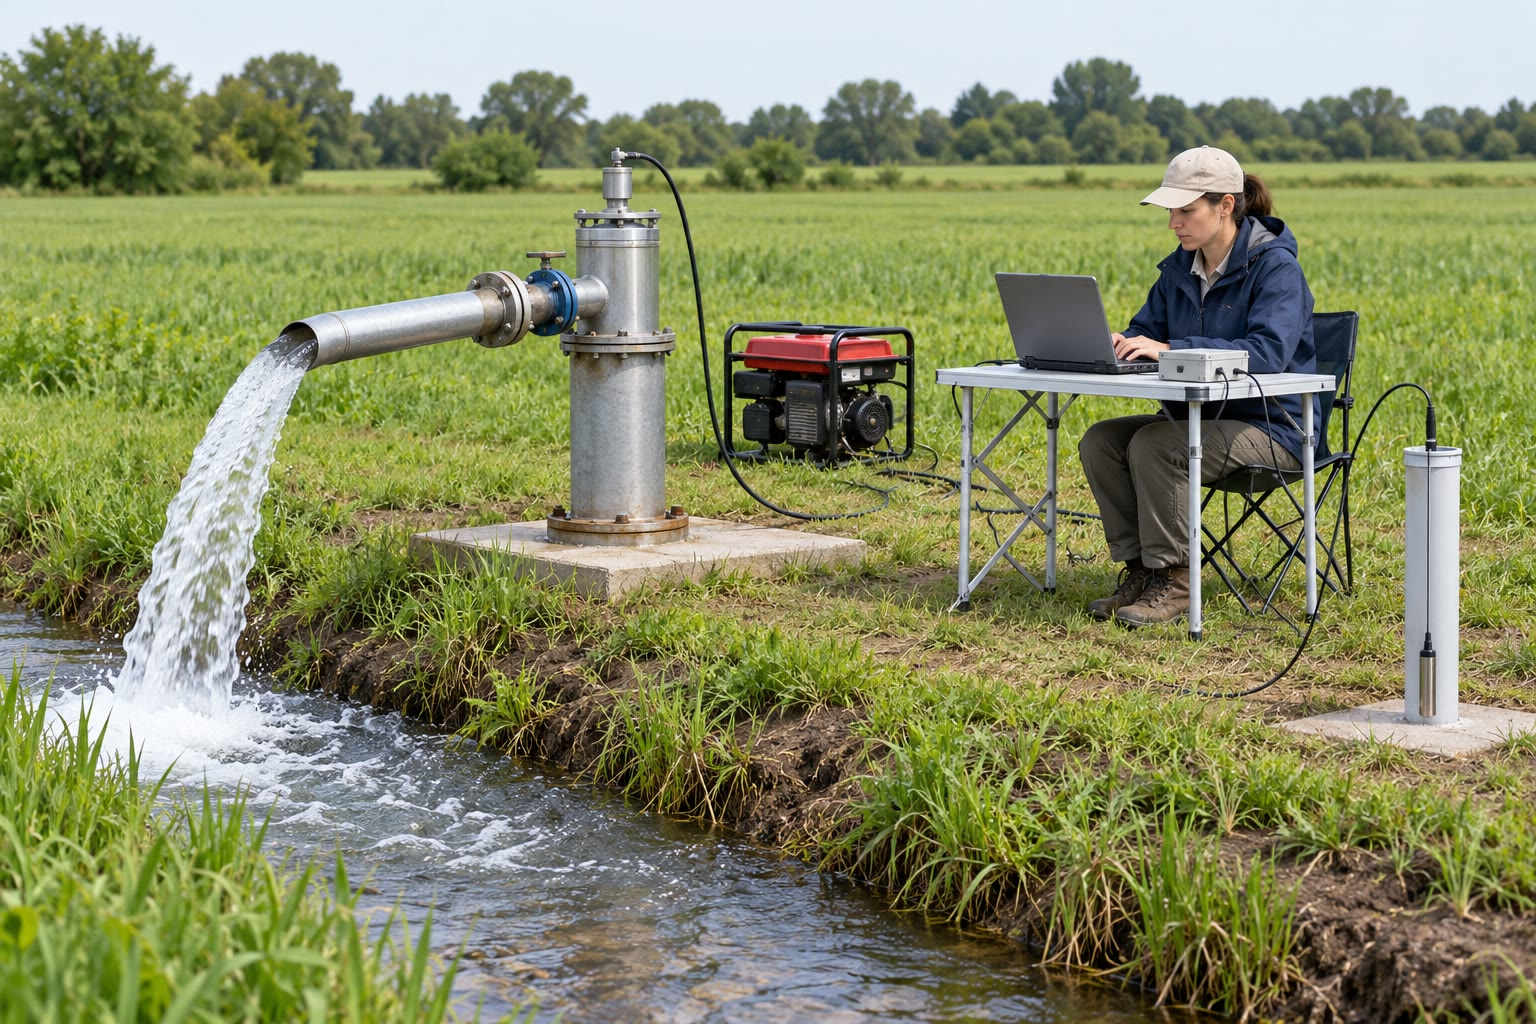
\includegraphics[width=\linewidth]{images/book5/ai/b3-pumping-test.jpg}

{\scriptsize Un essai de pompage~: la conduite de refoulement du puits pompé, un
groupe électrogène et un hydrogéologue qui relève les niveaux d'un puits
d'observation sur un ordinateur portable (Illustration générée par IA.)}
\end{minipage}
\end{inthefield}
% ledger: heath:theis, heath:jacob, heath:water-levels, usgs:transducers

\section{Transport de soluté}\label{sec:b3:hydrogeology:transport}

Un soluté dissous dans l'eau souterraine est entraîné avec l'eau, à la
\omterm{def:b3:hydrogeology:seepage}{vitesse effective}, et il se disperse au fil de son déplacement~: l'eau des
pores voisins se déplace à des vitesses différentes et suit des trajets
différents, et le soluté diffuse également.

\begin{definition}[Dispersion hydrodynamique~; dispersivité]\label{def:b3:hydrogeology:ade}
La \emph{dispersion hydrodynamique}\index{dispersion hydrodynamique} est
l'étalement d'un soluté dans une eau souterraine en écoulement, dû aux
variations de la vitesse de l'eau d'un pore à l'autre et à la diffusion
moléculaire. Le long de l'écoulement, elle se décrit par un coefficient de dispersion $D = \alpha_Lv + D^*$,
où $v$ est la \omterm{def:b3:hydrogeology:seepage}{vitesse effective}, $D^*$ la diffusivité moléculaire effective et
$\alpha_L$, une longueur, la
\emph{dispersivité}\index{dispersivité} longitudinale du milieu.
\end{definition}

\begin{theorem}[Équation d'advection--dispersion]\label{thm:b3:hydrogeology:ade}
Le long d'un écoulement unidimensionnel de \omterm{def:b3:hydrogeology:seepage}{vitesse effective} constante $v$, la
concentration $C(x, t)$ d'un soluté non réactif obéit à
\[
\frac{\partial C}{\partial t} = D\,\frac{\partial^2C}{\partial x^2} -
v\,\frac{\partial C}{\partial x} .
\]
Si la concentration est maintenue à $C_0$ en $x = 0$ à partir de $t = 0$, dans un
milieu initialement exempt de soluté,
\[
\frac{C}{C_0} = \frac12\left[\operatorname{erfc}\frac{x - vt}{2\sqrt{Dt}} +
\mathrm e^{vx/D}\operatorname{erfc}\frac{x + vt}{2\sqrt{Dt}}\right] .
\]
\end{theorem}
\index{equation d'advection--dispersion@équation d'advection--dispersion}

\begin{proof}
Dans une tranche de section unitaire et de longueur $\mathrm dx$, de porosité
efficace $n_e$, le soluté stocké vaut $n_eC\,\mathrm dx$. Son flux vaut
$n_e(vC - D\,\partial C/\partial x)$, entraîné avec l'eau et dispersé comme la
loi de Fick disperse une substance qui diffuse. La conservation donne
$n_e\partial_tC = -\partial_x[n_e(vC - D\partial_xC)]$, c'est-à-dire l'équation. Que la
formule la satisfasse ainsi que les conditions est admis ici~;
l'\cref{exo:b3:hydrogeology:12} en vérifie l'étalement.
\end{proof}

Dans le référentiel qui se déplace avec l'eau, $\xi = x - vt$, l'équation est
l'équation de diffusion, et le front s'étale comme $\sqrt{2Dt} = \sqrt{2\alpha_L
vt} = \sqrt{2\alpha_Lx}$~: la largeur du front croît comme la racine carrée
de la distance parcourue.

\begin{definition}[Facteur de retard]\label{def:b3:hydrogeology:retardation}
Un soluté adsorbé sur les grains, à l'équilibre et en proportion
à sa concentration, se déplace plus lentement que l'eau. Son
\emph{facteur de retard}\index{facteur de retard (sorption)} est
\[
R = 1 + \frac{\rho_bK_d}{n} ,
\]
$\rho_b$ étant la masse volumique apparente sèche du milieu, $n$ sa porosité et
$K_d$ le coefficient de distribution, c'est-à-dire la masse adsorbée par unité de masse de
solide divisée par la concentration dans l'eau. Le soluté se déplace à $v/R$
et se disperse avec $D/R$.
\end{definition}

\begin{omfigure}
\begin{tikzpicture}
\begin{groupplot}[group style={group size=2 by 1, horizontal sep=1.5cm},
  width=0.48\linewidth, height=0.4\linewidth,
  tick label style={font=\scriptsize}, label style={font=\small}, title style={font=\small}]
\nextgroupplot[xlabel={temps (jours)}, ylabel={$C/C_0$ à \qty{100}{m}},
  xmin=0, xmax=1000, ymin=0, ymax=1.05, title={courbes de percée},
  legend style={font=\scriptsize, at={(0.97,0.03)}, anchor=south east}]
% computed in figdata/bachelor-3/advection_dispersion.py
\addplot[omDef, thick] table[x=t, y=c1] {figdata/out/bachelor-3-advection_dispersion-btc.dat};
\addlegendentry{$\alpha_L = \qty{1}{m}$}
\addplot[omMeth, thick] table[x=t, y=c3] {figdata/out/bachelor-3-advection_dispersion-btc.dat};
\addlegendentry{$\alpha_L = \qty{3}{m}$}
\addplot[omThm, thick] table[x=t, y=c10] {figdata/out/bachelor-3-advection_dispersion-btc.dat};
\addlegendentry{$\alpha_L = \qty{10}{m}$}
\addplot[black, thick, densely dashed, forget plot] table[x=t, y=cR] {figdata/out/bachelor-3-advection_dispersion-btc.dat};
\node[font=\scriptsize, anchor=west, align=left] at (axis cs:640,0.45) {$\alpha_L = \qty{3}{m}$,\\ $R = 3$};
\addplot[black!40, densely dotted, forget plot] coordinates {(200,0) (200,1.05)};
\nextgroupplot[xlabel={distance (\unit{m})}, ylabel={$C/C_0$ après 150 jours},
  xmin=0, xmax=160, ymin=0, ymax=1.05, title={profils},
  legend style={font=\scriptsize, at={(0.03,0.03)}, anchor=south west}]
\addplot[omDef, thick] table[x=x, y=c1] {figdata/out/bachelor-3-advection_dispersion-profile.dat};
\addlegendentry{$\alpha_L = \qty{1}{m}$}
\addplot[omMeth, thick] table[x=x, y=c3] {figdata/out/bachelor-3-advection_dispersion-profile.dat};
\addlegendentry{$\alpha_L = \qty{3}{m}$}
\addplot[omThm, thick] table[x=x, y=c10] {figdata/out/bachelor-3-advection_dispersion-profile.dat};
\addlegendentry{$\alpha_L = \qty{10}{m}$}
\addplot[black!40, densely dotted, forget plot] coordinates {(75,0) (75,1.05)};
\end{groupplot}
\end{tikzpicture}

\par\smallskip{\small Un soluté injecté en continu en $x = 0$ dans un
écoulement de \omterm{def:b3:hydrogeology:seepage}{vitesse effective} \qty{0.5}{m/d}. À gauche, la concentration
\qty{100}{m} en aval, en fonction du temps~: l'eau elle-même arrive après
200 jours (pointillés)~; plus la \omterm{def:b3:hydrogeology:ade}{dispersivité} est grande, plus tôt arrivent les premières
traces et plus tard la concentration maximale. Un soluté adsorbé avec $R =
3$ arrive trois fois plus tard. À droite, la concentration le long de l'écoulement après
150 jours, lorsque l'eau a parcouru \qty{75}{m}
(pointillés).}\label{fig:b3:hydrogeology:transport}
\end{omfigure}

Les \omterm{def:b3:hydrogeology:ade}{dispersivités} sont difficiles à mesurer et, en pratique, on les fixe souvent par
des règles empiriques. La plus ancienne prend la \omterm{def:b3:hydrogeology:ade}{dispersivité} longitudinale égale au dixième de
la longueur du panache. Une compilation de mesures de terrain publiée en
1992 montre que la \omterm{def:b3:hydrogeology:ade}{dispersivité} croît avec l'échelle de l'expérience,
que les valeurs fiables aux grandes échelles sont peu nombreuses, et qu'à une échelle donnée les
valeurs s'étalent sur deux ou trois ordres de grandeur.
% ledger: epa:dispersivity

\section{Exercices}

\begin{exercise}[$\star$]\label{exo:b3:hydrogeology:1}
Deux piézomètres sont installés côte à côte sur un terrain situé à \qty{120.0}{m} au-dessus du
datum. Le premier est crépiné à \qty{40}{m} de profondeur et son eau se tient
\qty{12.5}{m} sous le sol~; le second est crépiné à \qty{80}{m}
de profondeur, son eau se tient \qty{15.0}{m} sous le sol. Calculer la charge de
position, la charge de pression et la \omterm{def:b3:hydrogeology:head}{charge hydraulique} aux deux crépines. Dans quel sens
l'eau circule-t-elle entre elles, et sous quel gradient vertical~?
\end{exercise}

\begin{exercise}[$\star$]\label{exo:b3:hydrogeology:2}
Une colonne de sable de \qty{50}{cm} de long et \qty{10}{cm} de diamètre, avec $K =
\qty{12}{m/d}$ et une porosité efficace de 0.35, est parcourue par de l'eau sous une
différence de charge de \qty{30}{cm}. Calculer la \omterm{def:b3:hydrogeology:darcy}{vitesse de Darcy}, le débit
en litres par heure, et la \omterm{def:b3:hydrogeology:seepage}{vitesse effective}.
\end{exercise}

\begin{exercise}[$\star$]\label{exo:b3:hydrogeology:3}
Un calcaire a $K = \qty{2.5}{m/d}$ pour l'eau à \qty{10}{\celsius}
($\rho = \qty{999.7}{kg/m^3}$, $\mu = \qty{1.306e-3}{Pa.s}$). Calculer sa
\omterm{def:b3:hydrogeology:darcy}{perméabilité intrinsèque}, et sa \omterm{def:b3:hydrogeology:darcy}{conductivité hydraulique} pour l'eau à
\qty{20}{\celsius} ($\rho = \qty{998.2}{kg/m^3}$, $\mu =
\qty{1.002e-3}{Pa.s}$).
\end{exercise}
% ledger: nist:water

\begin{exercise}[$\star$]\label{exo:b3:hydrogeology:4}
Le calcaire de l'aquifère captif du forage Varden-3 a une épaisseur de \qty{180}{m}, avec $K =
\qty{2.5}{m/d}$. Calculer sa \omterm{def:b3:hydrogeology:storage}{transmissivité}, et le \omterm{def:b3:hydrogeology:storage}{coefficient d'emmagasinement}
que l'aquifère aurait si seule la dilatation de l'eau, \num{9e-7} par mètre
d'aquifère par mètre de charge, libérait de l'eau. Comparer avec $S = \num{2e-4}$.
\end{exercise}
% ledger: heath:storage

\begin{exercise}[$\star\star$]\label{exo:b3:hydrogeology:5}
Après une longue période de pompage à \qty{1500}{m^3/d}, les rabattements ont
cessé d'évoluer~: \qty{2.35}{m} dans un puits d'observation situé à \qty{20}{m} du
puits pompé et \qty{0.82}{m} dans un autre situé à \qty{200}{m}. L'aquifère est
captif et épais de \qty{40}{m}. Calculer sa \omterm{def:b3:hydrogeology:storage}{transmissivité} et sa
\omterm{def:b3:hydrogeology:darcy}{conductivité hydraulique}.
\end{exercise}

\begin{exercise}[$\star\star$]\label{exo:b3:hydrogeology:6}
Un puits pompe \qty{1200}{m^3/d} dans un aquifère captif de $T =
\qty{300}{m^2/d}$ et $S = \num{5e-4}$. Calculer $u$, $W(u)$ (à partir de la
série), et le rabattement à \qty{300}{m} de distance, après 1 jour puis après 10 jours.
\end{exercise}

\begin{exercise}[$\star\star$]\label{exo:b3:hydrogeology:7}
Pour l'essai de Varden-3 ($T = \qty{450}{m^2/d}$, $S = \num{2e-4}$), au bout de
combien de minutes la droite de Cooper--Jacob peut-elle être utilisée dans les puits
d'observation situés à \qty{60}{m} et \qty{500}{m} du puits pompé~? Que dit cela
de l'emplacement des puits d'observation d'un essai de courte durée~?
\end{exercise}

\begin{exercise}[$\star\star$]\label{exo:b3:hydrogeology:8}
Deux puits distants de \qty{400}{m} dans le calcaire de Varden pompent chacun
\qty{2160}{m^3/d}. Calculer le rabattement après 10 jours à mi-distance entre eux,
puis au site du second puits, dû au seul premier puits. Pourquoi le pompage de chaque puits
coûte-t-il de l'argent à l'autre~?
\end{exercise}

\begin{exercise}[$\star\star$]\label{exo:b3:hydrogeology:9}
Dans le \omterm{def:b3:hydrogeology:flow-net}{réseau d'écoulement} sous le barrage, compter les tubes de courant et les chutes de charge.
Avec $K = \qty{5}{m/d}$ et $H = \qty{10}{m}$, calculer la perte par infiltration par
mètre de barrage, puis sous un barrage long de \qty{300}{m}.
\end{exercise}

\begin{exercise}[$\star\star\star$]\label{exo:b3:hydrogeology:10}
Modéliser un sable propre par des tubes droits de rayon \qty{50}{\micro\metre} et de
porosité de 0.30. Calculer $k$ et $K$ (pour l'eau à \qty{20}{\celsius}, comme dans
l'\cref{exo:b3:hydrogeology:3}),
et comparer avec la fourchette du sable propre. Quelles caractéristiques d'un sable réel
le modèle laisse-t-il de côté, et dans quel sens chacune fait-elle varier $K$~?
\end{exercise}
% ledger: nist:water, heath:k-chart

\begin{exercise}[$\star\star\star$]\label{exo:b3:hydrogeology:11}
(a)~Montrer que le rabattement de Cooper--Jacob s'annule en $r_0 =
\sqrt{2.25\,Tt/S}$. (b)~Calculer $r_0$ après 30 jours de pompage dans le
calcaire de Varden captif, puis pour la même roche à nappe libre, avec $S =
0.2$. (c)~Pourquoi le cône d'un aquifère captif peut-il atteindre une limite que l'essai
n'était pas censé détecter~?
\end{exercise}
% ledger: heath:jacob, heath:storage

\begin{exercise}[$\star\star\star$]\label{exo:b3:hydrogeology:12}
(a)~Pour une longue distance de parcours, la courbe de percée en $x$ est proche d'une
loi normale en temps, de moyenne $x/v$ et d'écart type $\sigma_t
= \sqrt{2\alpha_Lx}/v$. Le montrer à partir de l'étalement $\sqrt{2Dt}$ du front.
(b)~À \qty{100}{m}, avec $v = \qty{0.5}{m/d}$, la concentration atteint
\qty{16}{\percent} après \num{152.6}~jours et \qty{84}{\percent} après
\num{247.2}~jours. Estimer $\alpha_L$. (c)~Un aquifère sableux a $\rho_b =
\qty{1.9}{g/cm^3}$ et $n = 0.30$~; un soluté a $K_d =
\qty{0.32}{cm^3/g}$. Calculer $R$.
\end{exercise}

\section{Problème~: essai de pompage à Varden-3}

\begin{problem}[{Problème du week-end --- charges, essai de pompage et transport
d'un polluant dans le calcaire captif des collines de Varden}]
\label{pb:b3:hydrogeology:1}
Le puits fictif Varden-3 est foré en (4500, 5000) sur le quadrillage des
collines de Varden, à partir d'une cote du terrain de \qty{363.2}{m}, à travers
les argiles jurassiques jusqu'au calcaire jurassique, dont le toit se situe à
\qty{282.5}{m} et la base à \qty{102.5}{m} au-dessus du niveau de la mer~; le puits est ouvert
sur toute l'épaisseur du calcaire. Avant l'essai, l'eau y stationne
à \qty{45.0}{m} sous le sol.

\medskip\noindent\textbf{Partie I --- L'aquifère et son écoulement naturel.}
\begin{enumerate}
\item Calculer l'épaisseur des argiles et celle du calcaire au niveau du puits.
\item Calculer la charge dans le calcaire et la pression de charge au toit de celui-ci.
  Pourquoi le calcaire est-il ici un aquifère captif~?
\item Trois piézomètres ouverts dans le calcaire se trouvent en P1 (4300, 5250), P2
  (4850, 5150) et P3 (4550, 4650), avec des charges de 318.96, 317.34 et
  \qty{317.52}{m}. En posant $h = ax + by + c$, déterminer $a$ et $b$.
\item Calculer le \omterm{def:b3:hydrogeology:head}{gradient hydraulique} ainsi que l'azimut vers lequel
  s'écoule l'eau.
\end{enumerate}

\medskip\noindent\textbf{Partie II --- L'essai de pompage.} Le puits est pompé
à \qty{2160}{m^3/d} pendant deux jours. Dans un puits d'observation situé à \qty{60}{m}
de distance, les rabattements sont~:
\begin{center}
\begin{tabular}{l*{11}{c}}
\hline
$t$ (\unit{min}) & 1 & 2 & 3 & 5 & 7 & 10 & 15 & 20 & 30 & 45 & 60\\
$s$ (\unit{m}) & 0.18 & 0.36 & 0.48 & 0.64 & 0.77 & 0.88 & 1.04 & 1.15 & 1.30 & 1.45 & 1.56\\
\hline
$t$ (\unit{min}) & 90 & 120 & 180 & 240 & 360 & 480 & 720 & 960 & 1440 & 2160 & 2880\\
$s$ (\unit{m}) & 1.71 & 1.82 & 1.98 & 2.08 & 2.24 & 2.35 & 2.50 & 2.61 & 2.77 & 2.92 & 3.03\\
\hline
\end{tabular}
\end{center}
\begin{enumerate}[resume]
\item Tracer $s$ en fonction de $\log_{10}t$. Quels premiers points s'écartent de la
  droite, et pourquoi~?
\item Sur la partie rectiligne, mesurer le rabattement par cycle logarithmique.
\item Calculer la \omterm{def:b3:hydrogeology:storage}{transmissivité}.
\item Déterminer le temps $t_0$ auquel la droite coupe le rabattement nul.
\item Calculer le \omterm{def:b3:hydrogeology:storage}{coefficient d'emmagasinement}.
\item Vérifier que $u \le 0.05$ pour les points utilisés.
\item Calculer la \omterm{def:b3:hydrogeology:darcy}{conductivité hydraulique} du calcaire.
\end{enumerate}

\medskip\noindent\textbf{Partie III --- Le cône.} À partir d'ici, prendre $T =
\qty{450}{m^2/d}$ et $S = \num{2e-4}$.
\begin{enumerate}[resume]
\item Calculer le rabattement de Theis dans le puits d'observation après 2 jours et
  le comparer à la mesure.
\item Un puits agricole situé à \qty{1}{km} puise dans le même calcaire. Calculer son
  rabattement après 30 jours de pompage.
\item Calculer la distance $r_0$ de Jacob après 30 jours. Que dit-elle à propos des
  bords de l'aquifère et de la faille des collines de Varden~?
\item Calculer le volume pompé en 30 jours. Dans un aquifère captif, d'où
  provient-il~?
\item Comment le rabattement à la ferme se comparerait-il si le calcaire était
  à nappe libre, avec $S = 0.18$~?
\end{enumerate}

\medskip\noindent\textbf{Partie IV --- Un polluant.} Une fuite d'un polluant dissous
atteint le calcaire à \qty{200}{m} du puits. Prendre une porosité efficace de
0.18 et un \omterm{def:b3:hydrogeology:retardation}{facteur de retard} de 2.5.
\begin{enumerate}[resume]
\item Avant le pompage, calculer la \omterm{def:b3:hydrogeology:darcy}{vitesse de Darcy} et la \omterm{def:b3:hydrogeology:seepage}{vitesse effective}
  de l'écoulement naturel de la partie~I.
\item Combien de temps l'eau mettrait-elle pour parcourir \qty{200}{m}, et le
  polluant~?
\item Le puits pompant et la fuite étant en amont de celui-ci, l'écoulement
  devient radial vers le puits. Montrer que l'eau met $t = \pi n_e b
  r^2/Q$ pour atteindre le puits depuis une distance $r$, en négligeant l'écoulement
  naturel, et calculer ce temps pour l'eau et pour le polluant.
\item Avec la règle empirique d'une \omterm{def:b3:hydrogeology:ade}{dispersivité} égale au dixième de la distance,
  estimer l'étalement $\sqrt{2\alpha_Lx}$ du front au puits. Que
  signifie-t-il pour la première arrivée~?
\item Faut-il poursuivre le pompage~? Donner un argument pour et un contre.
\item Donner la \omterm{def:b3:hydrogeology:storage}{transmissivité} de l'aquifère du calcaire de Varden, en mètres carrés par
  jour, à deux chiffres significatifs près.
\end{enumerate}
\end{problem}
% ledger: heath:jacob, heath:theis, heath:storage, epa:dispersivity, region:name
